\documentclass[letter, 10pt]{article}
\usepackage[spanish]{babel}
\usepackage[utf8]{inputenc} 
\usepackage[T1]{fontenc}
\usepackage{lmodern}
\usepackage{amsfonts}
\usepackage{amsmath}
\usepackage{graphicx}
\usepackage{url}
\usepackage{listings}
\usepackage[top=3cm,bottom=3cm,left=3.5cm,right=3.5cm,footskip=1.5cm,headheight=1.5cm,headsep=.5cm,textheight=3cm]{geometry}


\begin{document}
\title{Inteligencia Artificial \\ \begin{Large}Estado del Arte: Green-Vehicle Routing Problem (G-VRP)\end{Large}}
\author{Paula Pérez}
\date{2020}
\maketitle


\begin{abstract}
Muchos problemas de optimización clásicos provienen del área productiva, donde se busca ahorrar en costos de producción, transporte, logística a través de modificar parámetros operacionales. La preocupación medioambiental en los últimos años ha propiciado la inclusión de nuevas restricciones en las metas productivas, las cuales han diversificado el escenario de soluciones posibles para cumplir con estas regulaciones. Así, problemas como el \textit{Green Vehicle Routing Problem} (G-VRP), el cual busca minimizar la distancia de una flota bajo vigilancia del uso de combustible, se ha vuelto interesante y ha sido sometido a una extensa investigación en las ultimas décadas. Este reporte revisa los algoritmos de solución empleados en G-VRP para diferentes números de parámetros, realizando un compromiso entre exactitud de la solución y la factibilidad computacional para los casos a gran escala. 

\end{abstract}

\section{Introducci\'on}
El \textit{Green-Vehicle Routing Problem} (G-VRP), variante del \textit{Vehicle Routing Problem} (VRP), busca ayudar a una flota de vehículos de combustible alternativo para cumplir con los requerimientos de un conjunto de clientes, minimizando la distancia total viajada de todos los vehículos. Este tipo de problemas y su solución son importantes para empresas de transporte, ya que permite ahorrar de forma significativa en insumos y gastos base. Formalmente fue tratado inicialmente en 2012 y ha suscitado una linea de investigación que continua hasta hoy, debido a la creciente inclusión de tecnologías limpias en los procesos productivos. A modo de resumen, se definirá y conceptualizará el problema de manera general. También se detallará su estado del arte actual, mencionando las metodologías frecuentemente utilizadas en la literatura. Posteriormente se presentará el modelo matemático que representa el problema, sus objetivos y variables para finalmente concluir acerca de la información recopilada y cual son las prospecciones para enfrentar este problema en sistemas a mayor escala, lo cual se observa hoy en día en empresas multinacionales.
\section{Definici\'on del Problema}

 El \textit{Green-Vehicle Routing Problem} (G-VRP) es una variante del \textit{Vehicle Routing Problem} (VRP) documentado por primera vez por Erdoğan y Miller-Hooks en el año 2012~\cite{erdogan_green_2012}. Lenstra y Rinnooy Kan demostraron en 1981 que el problema VRP es un problema NP-duro. Como el problema VRP es un caso particular del problema G-VRP, es posible concluir que el problema \textit{Green-Vehicle Routing Problem} es también NP-duro~\cite{montoya_multi-space_2016}.
 \\El clásico \textit{Vehicle Routing Problem} (VRP) busca ayudar a una flota de vehículos en una red dada a servir a un conjunto de clientes bajo restricciones relacionadas a la demanda y los suministros, usualmente minimizando la distancia total viajada de todos los vehículos o minimizando los costos asociados a los viajes. Usualmente el costo se calcula como una función lineal respecto a la distancia~\cite{koc_green_2016}. El \textit{Green-Vehicle Routing Problem} como variante de este problema, considera la utilización de combustibles alternativos, agrega como variable el consumo de combustible de los vehículos y añade puntos de recarga de combustible en las rutas, manteniendo como objetivo la minimización de la distancia total viajada por los vehículos, y en consecuencia los costos totales asociados.~\cite{erdogan_green_2012}
 \\El \textit{Green-Vehicle Routing Problem} (G-VRP) está formulado como programación lineal en enteros mixta (PLEM). Dado un grafo completo cuyos vértices representan la ubicación de los clientes, los puntos de recarga de combustible alternativo y el depósito, el G-VRP busca un conjunto de rutas de distancia mínima posible que comience en el depósito, visite a un conjunto de clientes dentro de un tiempo límite preestablecido y regrese al depósito sin exceder el rango de distancia máxima recorrida del vehículo que depende de la capacidad de su tanque de combustible. Cada ruta puede incluir una o más paradas a los puntos de recarga de combustible alternativo, para que el vehículo pueda recargar combustible durante la ruta.~\cite{erdogan_green_2012}
 \\Algunas variantes existentes del problema son:
 \begin{itemize}
     \item \textit{Electric Vehicle Routing Problem with Time Windows an Recharge Stations} (E-VRPTW): Variante para vehículos eléctricos, se considera un tiempo de recarga dependiente del nivel de batería del vehículo. Cada cliente debe ser servido dentro de un margen de tiempo determinado. Los clientes requieren cantidades específicas de producto, se considera la capacidad de carga del vehículo.~\cite{Electric}
     \item \textit{Green Vehicle Routing Problem with Multiple Technologies and Partial Recharge} (GVRP-MTPR): Variante que incluye distintas tecnologías de recarga de estaciones de servicio. El tiempo de recarga parcial de combustible varía. Se admite una recarga parcial de combustible. ~\cite{felipe_heuristic_2014}
     \item \textit{Vehicle Routing Problem with Intermediate Stops} (VRPIS): Los consumidores requieren cantidades específicas de producto. Se consideran las capacidades de carga de los vehículos. Además de los puntos de recarga de combustible, se añaden puntos de recarga de productos.~\cite{Intermediate}
 \end{itemize}
También merece mencionar cuales son los problemas que antecedieron al G-VRP y forman parte de una familia mas numeroso de problemas de optimización en producción. Entre ellos esta el Vehicle Routing Problem (VRP), descrito en 1959 por George Dantzig y John Ramser, que trata la optimización de costos en flotas de transporte. Este a su vez se puede considerar una generalización del ubicuo Travelling Salesman Problem (TSP), uno de los más estudiados en teoría de la computación. 

\section{Estado del Arte}
El problema es mencionado por primera vez en 2012 como una variante del \textit{Vehicle Routing Problem} (VRP)~\cite{erdogan_green_2012}, debido a la necesidad de adaptar el problema a nuevas problemáticas como el uso de combustibles alternativos, añadiendo nuevas posibilidades de acortar trayectos como la recarga de combustible. La primera metodología de resolución de este problema, \textit{clusterfirst route-second procedure} fue planteada por Erdoğan y Miller-Hooks~\cite{erdogan_green_2012}, siendo el primer ejemplo de un algoritmo heurístico para el problema. Se han mencionado en la literatura métodos exactos (basados en programación lineal), métodos híbridos y métodos metaheurísticos. En el primer caso, los métodos exactos, éstos han demostrado ser inadecuados para la resolución de problemas de optimización a gran escala~\cite{koc_green_2016}~\cite{bruglieri_more_2019}~\cite{bruglieri_new_2016}. Luego, con la introducción de los métodos metaheurísticos, la gama de soluciones se diversificó incluyendo novedosas estrategias híbridas ~\cite{zhang_meta-heuristic_2018}~\cite{yin_adaptive_2016}. Los algoritmos metaheurísticos gozan de menores requerimientos computacionales respecto a las soluciones exactas, lo que posibilita su uso a mayor escala. Gracias a esto se han vuelto el enfoque dominante para la resolución del problema~\cite{peng_memetic_2019}~\cite{asghari_green_2020}~\cite{moghdani_green_2021}. Dentro de esta categoría se destacan algoritmos de la colonia de hormigas o \textit{Ant colony optimization} (ACO), \textit{Large neighborhood search } (ALNS), algoritmos genéticos o \textit{Genetic algorithm} (GA), algoritmo de recocido simulado o \textit{Simulated annealing} (SA) y búsqueda tabú o \textit{Tabu search } (TS)~\cite{moghdani_green_2021}~\cite{asghari_green_2020}.
\\A continuación se muestra un esquema representativo de los tipos de metodologías presentes en la literatura.
\begin{center}
\begin{figure}[h!]
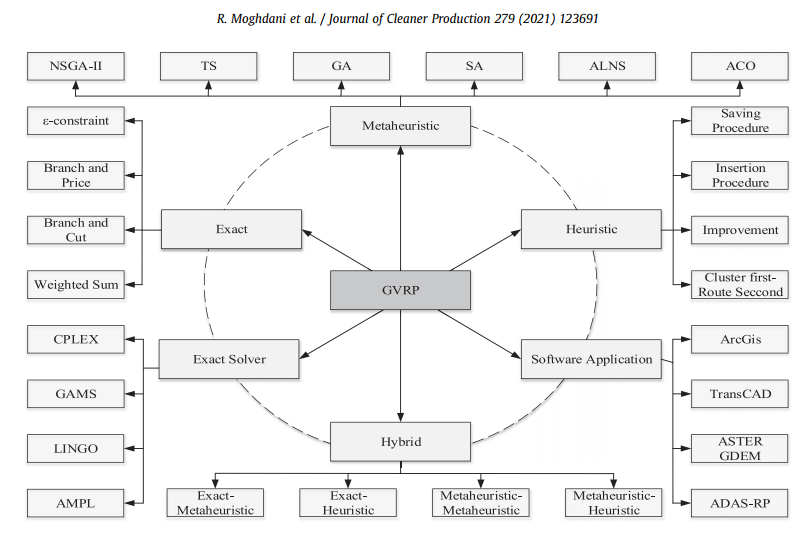
\includegraphics[width=1\textwidth]{paper1.PNG}
\caption{Marco general de las metodologías de resolución~\cite{moghdani_green_2021}.}
\end{figure}
\end{center}
Hasta la fecha no existe claridad sobre qué método presenta los mejores resultados, sin embargo, existe una tendencia hacia la aplicación de algoritmos metaheurísticos y estrategias híbridas.~\cite{moghdani_green_2021}}
\newpage El siguiente gráfico representa la frecuencia de las metodologías utilizadas en la resolución del problema presentes en la literatura.

\begin{center}
\begin{figure}[h!]
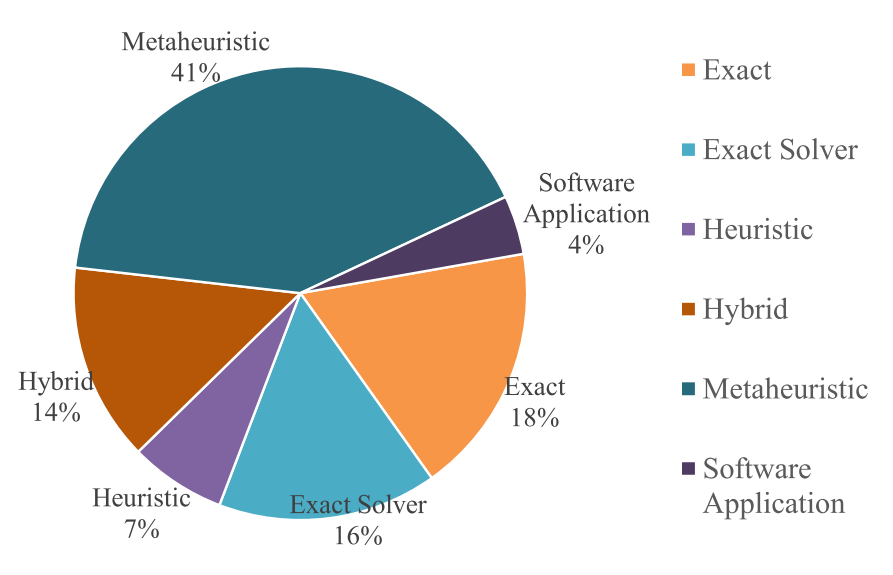
\includegraphics[width=0.8\textwidth]{paper2.PNG}
\caption{Porcentajes de las distintas metodologías de resolución en la literatura ~\cite{moghdani_green_2021}}
\end{figure}
\end{center}

Además de los distintos tipos de metodología utilizados para la resolución del problema, se ha visto en la literatura diversos enfoques con respecto al planteamiento de los objetivos del G-VRP~\cite{moghdani_green_2021}. Es posible observar que predomina el modelado del problema con un único objetivo, aunque se ha visto un leve aumento de los enfoques bi-objetivo, principalmente en las variantes de este problema~\cite{suzuki_dual-objective_2016}.
\begin{figure}[h]
\begin{center}
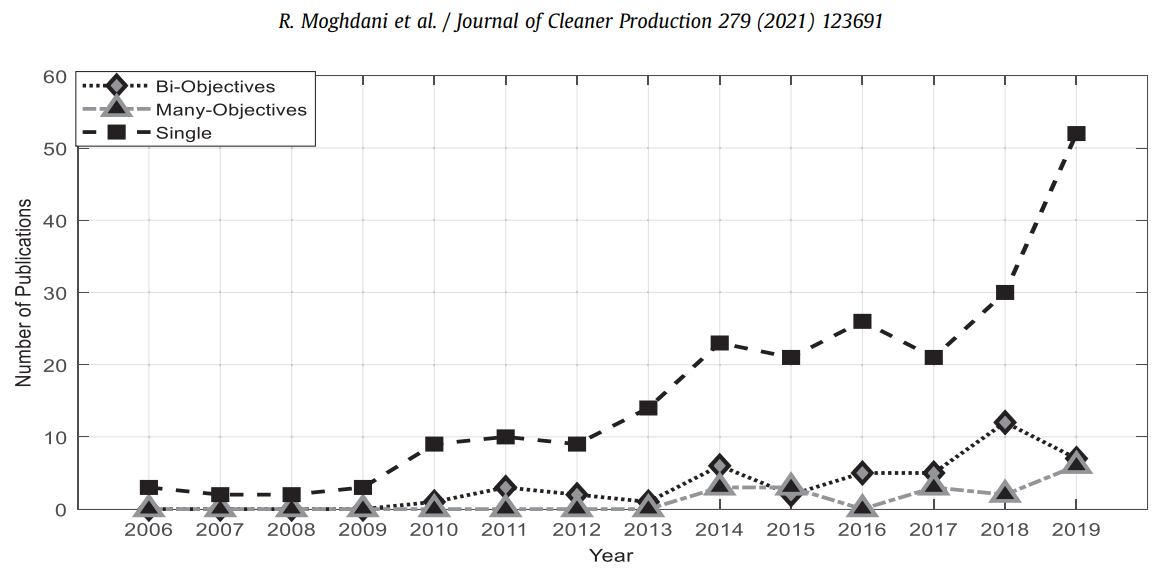
\includegraphics[width=0.8\textwidth]{paper3.PNG}\\
\caption{Distribución de cantidad de objetivos definida para el problema en publicaciones a lo largo de los años~\cite{moghdani_green_2021}}
\end{center}
\end{figure}

\section{Modelo Matem\'atico}
Modelo matemático propuesto por Erdoğan y Miller-Hooks~\cite{erdogan_green_2012}
\\ G-VRP se define como un grafo no dirigido $G=(V,E)$, donde $V$ corresponde al conjunto de vértices del grafo, que se compone por el conjunto de $n$ clientes $I$, el almacen $v_0$, y el conjunto $F$, con $s \geq 0$ estaciones de servicio.
\\En el conjunto $E$, cada arco se encuentra asociado a un tiempo $T_{ij}$, costo $c_{ij}$ y distancia $d_{ij}$.
\\Notación:
\begin{itemize}
    \item $I_0$ : Conjunto de vértices de consumidores y almacén, $I_0 = \{v_o\} \cup I$
    \item $F_0$ : Conjunto de vértices de estaciones de servicio y almacén, $F_0 = \{v_0\} \cup F'$
    \item $p_i$ : tiempo de servicio en el vértice $i$ ($t_c$ o $t_e$)
    \item $r$ : tasa de consumo de combustible
    \item $Q$ : Capacidad de combustible del tanque de los vehículos
    \item $T_{MAX}$ : Tiempo de conducción máximo por vehículo (TL)
    \item $m$ : Cantidad de vehículos
\end{itemize}
\textbf{Variables:}
\begin{itemize}
    \item $x_{ij}= \begin{cases} 
     \text{1} &\quad\text{Si el vehículo viaja desde el vértice}\\
       \text{0} &\quad\text{En caso contrario}\\
       \end{cases}$
    \item $y_j = $ Variable de nivel de combustible que especifica el nivel de combustible restante del tanque al llegar al vértice $j$. Se reajusta a $Q$ en cada vértice de estación de servicio $i$, y en el almacén.
    \item $\tau_j = $ Variable de tiempo que especifica el tiempo de llegada de un vehículo al vértice $j$, inicializada en cero a la salida del almacén.
\end{itemize}
\textbf{Función Objetivo:}
\begin{align*}
mín \sum_{i,j \in V', i \neq j} d_{ij}x_{ij}    
\end{align*}
\textbf{Restricciones:}\\
\\
Desde un vértice consumidor, se debe ir necesariamente a un solo otro vértice que sea consumidor, estación de servicio o almacén:
\begin{align}
     \sum_{j \in V', j \neq i} x_{ij} = 1, \forall i \in I 
\end{align}
Desde un vértice de estación de servicio, se puede ir a lo más a un solo otro vértice que sea consumidor, estación de servicio , o almacén:
\begin{align}
     \sum_{j \in V', j \neq i} x_{ij} \leq 1, \forall i \in F_0 
\end{align}
La cantidad de llegadas y partidas debe ser la misma para todos los vértices:
\begin{align}
    \sum_{j \in V' j \neq i} x_{ji} - \sum_{j \in V' j \neq i} x_{ij} = 0, \forall j \in V'
\end{align}
A lo más $m$ vehículos pueden salir desde el almacén:
\begin{align}
    \sum_{j \in V' \backslash \{0\}} x_{0j} \leq m
\end{align}
A lo más $m$ vehículos pueden llegar al almacén:
\begin{align}
    \sum_{j \in V' \backslash \{0\}} x_{j0} \leq m
\end{align}
El tiempo de llegada a cada vértice por cada vehículo es rastreado a través de la restricción (6). Las restricciones (6), (7) y (8) aseguran que cada vehículo vuelva al almacén a más tardar en $T_{MAX}$.
\begin{align}
    \tau_j \geq \tau_i + (t_{ij} - p_j )x_{ij} - T_{MAX}(1 - x_{ij}), i \in V' \backslash \{0\} \land i \neq j
    \\ 0 \leq \tau_0 \leq T_{MAX}
    \\ \tau_{0j} \leq \tau_j \leq T_{MAX} - (t_{j0} - p_j), \forall j \in V' \backslash \{0\}
\end{align}
Cada vez que se avance entre 2 vértices, si se llega a un consumidor, se debe disminuir la cantidad de combustible en base a la distancia recorrida:
\begin{align}
    y_j \leq y_i - r \dot d_{ij}x_{ij} + Q(1-x_{ij}), \forall j \in I \land i \in V', i \neq j
\end{align}
Si se llega a una estación de servicio o almacén, el combustible se restablece a $Q$:
\begin{align}
    y_j = Q, \forall j \in F_0
\end{align}
Se debe asegurar el retorno al almacén ya sea por vértices consumidores, o pasando por una estación de servicio:
\begin{align}
    y_j \geq mín\{ r \dot d_{j0}, r \dot (d_{jI} + d_{I0})\}, \forall j \in I, \forall I \in F'
\end{align}
La variable $x_{ij}$ solo puede tomar valores de 0 o 1:
\begin{align}
    x_{ij} \in \{ 0, 1\} \forall i,j
\end{align}
\section{Representación}
La representación del problema se basa en un arreglo bidimensional de enteros llamado \textit{visitas} sobre el cual opera, que indica con cuántas veces un nodo fue visitado por el vehículo $m$, en otras palabras, una lista de adyacencia. A través de este arreglo es posible manejar la restricción de que cada cliente sea visitado una única vez. No se utilizó un arreglo de booleanos debido a que los puntos de recarga de combustible pueden ser visitados más de una vez. Como el problema fue resuelto utilizando una técnica completa, se asumió una cantidad máxima de visitas a los puntos de recarga correspondiente a la cantidad de nodos de la instancia, ya que teniendo restricciones de tiempo, es improbable que una solución óptima contemple una mayor cantidad de visitas a cada uno de esos nodos. 
\begin{lstlisting}
    int **visitas;
\end{lstlisting}
Un arreglo bidimensional de enteros llamado \textit{recorrido} registra el orden de las rutas de cada vehículo \textit{m} a cada iteración a través de el identificador de cada nodo. Un arreglo de las mismas dimensiones llamado \textit{recorrido\_final} guarda el mejor recorrido a cada iteración.
\begin{lstlisting}
    vector <vector <int>> recorrido;
    vector <vector <int>> recorrido_final;
\end{lstlisting}
Cada nodo del grafo completo está representado por un objeto de clase \textit{Nodo} que contiene un identificador que lo caracteriza, un nombre, un tipo, y dos coordenadas que indican latitud y longitud. Todos estos parámetros son entregados al inicio del programa por la instancia correspondiente. Esta clase permite manejar los atributos de cada nodo de manera clara, legible y ordenada.
\begin{lstlisting}
class Nodo {
    public:
    int Id;
    string label;
    char Type;
    double Longitude;
    double Latitude;
    Nodo(int id, string descripcion, char tipo, double longitud, 
    double latitud){
      Id = id;                // ID que representa al nodo
      label = descripcion;    // Nombre del nodo en la instancia
      Type = tipo;            // Tipo del nodo 
                                (deposito, punto de recarga o cliente)
      Longitude = longitud;   // Longitud donde se encuentra el nodo
      Latitude = latitud;     // Latitud donde se encuentra el nodo
    }
    Nodo() = default;
};
\end{lstlisting}
Los nodos son guardados de manera ordenada en un arreglo de nodos llamado \textit{nodos}, de este modo se puede acceder a sus atributos únicamente mediante su identificador:
\begin{lstlisting}
    Nodo *nodos;
\end{lstlisting}
La distancia entre cada uno de los nodos se calcula a través de la función de Harvesine~\cite{erdogan_green_2012}, y es almacenada en un arreglo bidimensional de flotantes para no volver a calcularla a cada iteración:
\begin{lstlisting}
    double **distancias;
\end{lstlisting}
Las restricciones de combustible y tiempo máximo, se controlan mediante un registro de los valores actuales de nivel de gasolina y tiempo por vehículo a cada iteración. Estos valores se almacenan en arreglos, donde cada posición corresponde a un vehículo de manera ordenada.
\begin{lstlisting}
    double *gasolina;
    double *tiempo;
\end{lstlisting}
La función objetivo del modelo matemático se maneja a través de la variable flotante \textit{ans}, que registra la distancia mínima que cumple con las restricciones a cada iteración. Como se busca minimizar, la variable se inicializa con el máximo valor posible.
\begin{lstlisting}
    double ans = __DBL_MAX__;
\end{lstlisting}


\section{Descripción del algoritmo}
El algoritmo corresponde a un \textit{Backtracking} recursivo, es decir una técnica competa, utilizando las técnicas de \textit{Conflict Backjumping} (CBJ) y \textit{Forward Checking} (FC). 
A continuación se presenta el pseudocódigo del algoritmo.
\begin{lstlisting}
G-VRP(visitas, solucion, nodos, distancias, gasolina, tiempo, parametros, 
posicion_actual, registro_de_pasos, conflictos){

    si (se visitaron a todos los clientes, el recorrido empieza y termina 
    en el deposito y la distancia es menor a la solucion actual):
    
        solucion actual = nueva solucion;
        
    Luego de terminar de iterar:
    
        return;
        
    por cada vehiculo:
        por cada nodo:
            si(se cumplen las restricciones de tiempo, gasolina y 
            numero maximo de visitas):
            
                Se marca el nodo como visitado;
                
                registro_de_pasos.append(movimientos);
                
                G-VRP(visitas, solucion, nodos, distancias, gasolina, 
                tiempo, parametros, indice_nodo_actual, 
                registro_de_pasos, conflictos);
                
                Se marca el nodo como no visitado;
                
            else:
                Se añade el nodo anterior a la lista de conflictos 
                del nodo actual si es que no esta en ella;
                
                si(la lista de conflictos esta llena):
                    Se agregan los nodos de la lista de conflictos del 
                    nodo actual
                    al nodo anterior con el que tuvo conflicto;
                    
                    Se vuelve al ultimo nodo con el que tuvo conflicto; 
}
\end{lstlisting}
A cada iteración se comprueba que el movimiento es factible para instanciar el siguiente nodo.
El FC ocurre a través de la lista de adyacencia por vehículo, debido a que una vez que marca un nodo como visitado por un vehículo, no se probarán los casos en los que los otros vehículos pasen por ese nodo para esa instanciación.
El CBJ ocurre cuando no se cumplen las restricciones para el movimiento, el último nodo instanciado se agrega a la lista de conflictos del nodo actual. Si la lista de conflictos está llena, se agregan los nodos de la lista de conflictos del nodo actual a la lista de conflictos del último nodo con el que se tuvo conflicto y se hace un \textit{backjumping} a ese nodo. Sin embargo, no pude concretar de manera eficaz esa técnica por lo que pese a que está incorporada en el código, los pasos correspondientes a esta técnica están comentados.
\section{Experimentos}
Para distintas instancias construidas a partir de las instancias pequeñas entregadas, de hasta de 10 nodos, se probó la eficacia y eficiencia del algoritmo. Sin embargo, el tiempo comenzó a aumentar exponencialmente a partir de los 6 nodos, sin embargo, debido a motivos de tiempo no fue posible incorporar en detalle estos resultados. A medida de que las instancias aumentan su tamaño, el tiempo de ejecución también lo hace de manera exponencial, al igual que los resultados obtenidos en el paper original ~\cite{erdogan_green_2012}.
\section{Resultados}
Al usar técnicas completas, las instancias pequeñas entregadas tuvieron un tiempo de ejecución mayor a las 6 horas, y las instancias grandes fueron imposibles de finalizar en un tiempo razonable.
\section{Conclusiones}
Múltiples estrategias se han propuesto para la resolución del \textit{Green-Vehicle Routing Problem} (G-VRP) y sus variantes.
Estas técnicas varían respecto a las consideraciones en el modelado de sus restricciones, la cantidad de objetivos a considerar y los algoritmos de resolución. 
Las metodologías de solución del problema tienden actualmente a la utilización de metaheurísticas y técnicas híbridas, sin embargo ningún método asegura hallar una solución óptima al G-VRP aplicado a gran escala. Uno de los enfoques más prometedores es el uso de hiperheurísticas, como forma de reforzar las técnicas híbridas y de lograr una rápida adaptación a las diversas variantes del problema.
\\
\\El uso de técnicas completas para este tipo de problema, puede resultar altamente ineficiente, debido al gran tiempo de cómputo y recursos que requiere. Las técnicas completas utilizadas para la resolución de este problema son muy similares al TSP, y una el enfoque hacia la resolución del problema utilizando técnicas incompletas resultaría una opción más factible.
\\
\\Queda trabajo por realizar a futuro, como el reforzar la investigación interdisciplinaria del problema para que la construcción matemática sea más realista y en este mismo sentido, la implementación de variables estocásticas para el modelado del problema bajo incertidumbre, ej. tiempo de servicio como una variable aleatoria. También, a modo de propuesta para continuar las investigaciones futuras, sería establecer una métrica(s) universal(es) de desempeño de las técnicas de resolución del problema para confrontarlas y evaluarlas objectivamente. 

\newpage
\section{Bibliograf\'ia}

\bibliographystyle{unsrt}
\bibliography{Referencias}

\end{document} 